
\chapter{协议实现}

第二周的协议实现主要分为“基本方法实现”、“缓冲区处理”、“日志记录模块”、“读写文件”和两个部分。

\section{方法实现}

服务器处理请求的方法被集中封装到文件 response.c 和 response.h 中。函数原型如图\ref{fig:Responsech} 所示。

具体而言,liso\_server 首先使用 while 来接收信息,存储到 buffer 中(此处采用自定义的动态缓存,在下一节详细介绍)。然后通过一个 strstr() 函数获取确定一个完整的请求后,将它加载到动态缓存 dbuf 中,并调用函数 handle\_request 处理,返回的信息将继续通过 dbuf 带出。由于测试集的要求,此处不需要实现 Persistent Connection 中对连接情况的判断。下面将分别介绍错误码和基本方法的实现。

\subsection{错误码}

\paragraph*{400}
400 错误是解析错误,由于之前在 Lab 1 已经实现了较为完备的 parse() 函数,于是在 Lab 2 中将不再 parse() 函数之内做修改。\textbf{首先},通过图\ref{fig:Responsech}左侧 第 37 行调用 parse() 函数对请求进行解析,并通过第 40 行的判断确定一个 400 的错误,并随即调用函数 handle\_400 处理之。\textbf{然后},通过对自定义函数的调用,对动态缓冲数组 dbuf 进行清空、加载返回信息等操作。

\paragraph*{404}
404 错误是指无法找到请求的文件,目前只会在 HEAD 和 GET 方法处理时出现。在处理 GET 和 HEAD 请求时,我们会通过 stat 等函数对要请求的文件进行预处理,此时即可判断该文件是否存在、是否可读等权限问题,然后决定是否返回 404 错误。

\paragraph*{505}
505 错误是指协议版本不支持,通过图\ref{fig:Responsech} 左侧第 53 行判断 my\_http\_version 与请求的 version 是否相同即可。

\paragraph*{501}

501 错误是指请求方法不支持,也可以通过一个 switch 判断出来。此处的 method\_switch() 函数,将一个表示方法的字符串 ("GET", "POST", etc) 转化为图\ref{fig:Responsech} 右侧第 35 行定义的枚举类 METHOD。


\subsection{基本方法}

\paragraph*{HEAD} HEAD 方法的具体实现由函数 handle\_head() 实现。\textbf{首先},通过函数 strcmp() 判断请求路径是否为默认路径,如果是,则直接请求文件 index.html, 否则请求路径添加到子文件夹 "./static\_site" 之下。\textbf{然后},通过函数 stat() 判断是否为 404 错误。如果一切顺利,则通过在下一节介绍的动态缓冲区处理函数按照前文提到的格式,向返回值 dbuf 中添加一系列 response 和 headers。具体如图\ref{fig:handleHead} 所示。


\begin{figure}[htbp!]
    \centering
    \subfigure[Response.c 和 Response.h]{\label{fig:Responsech}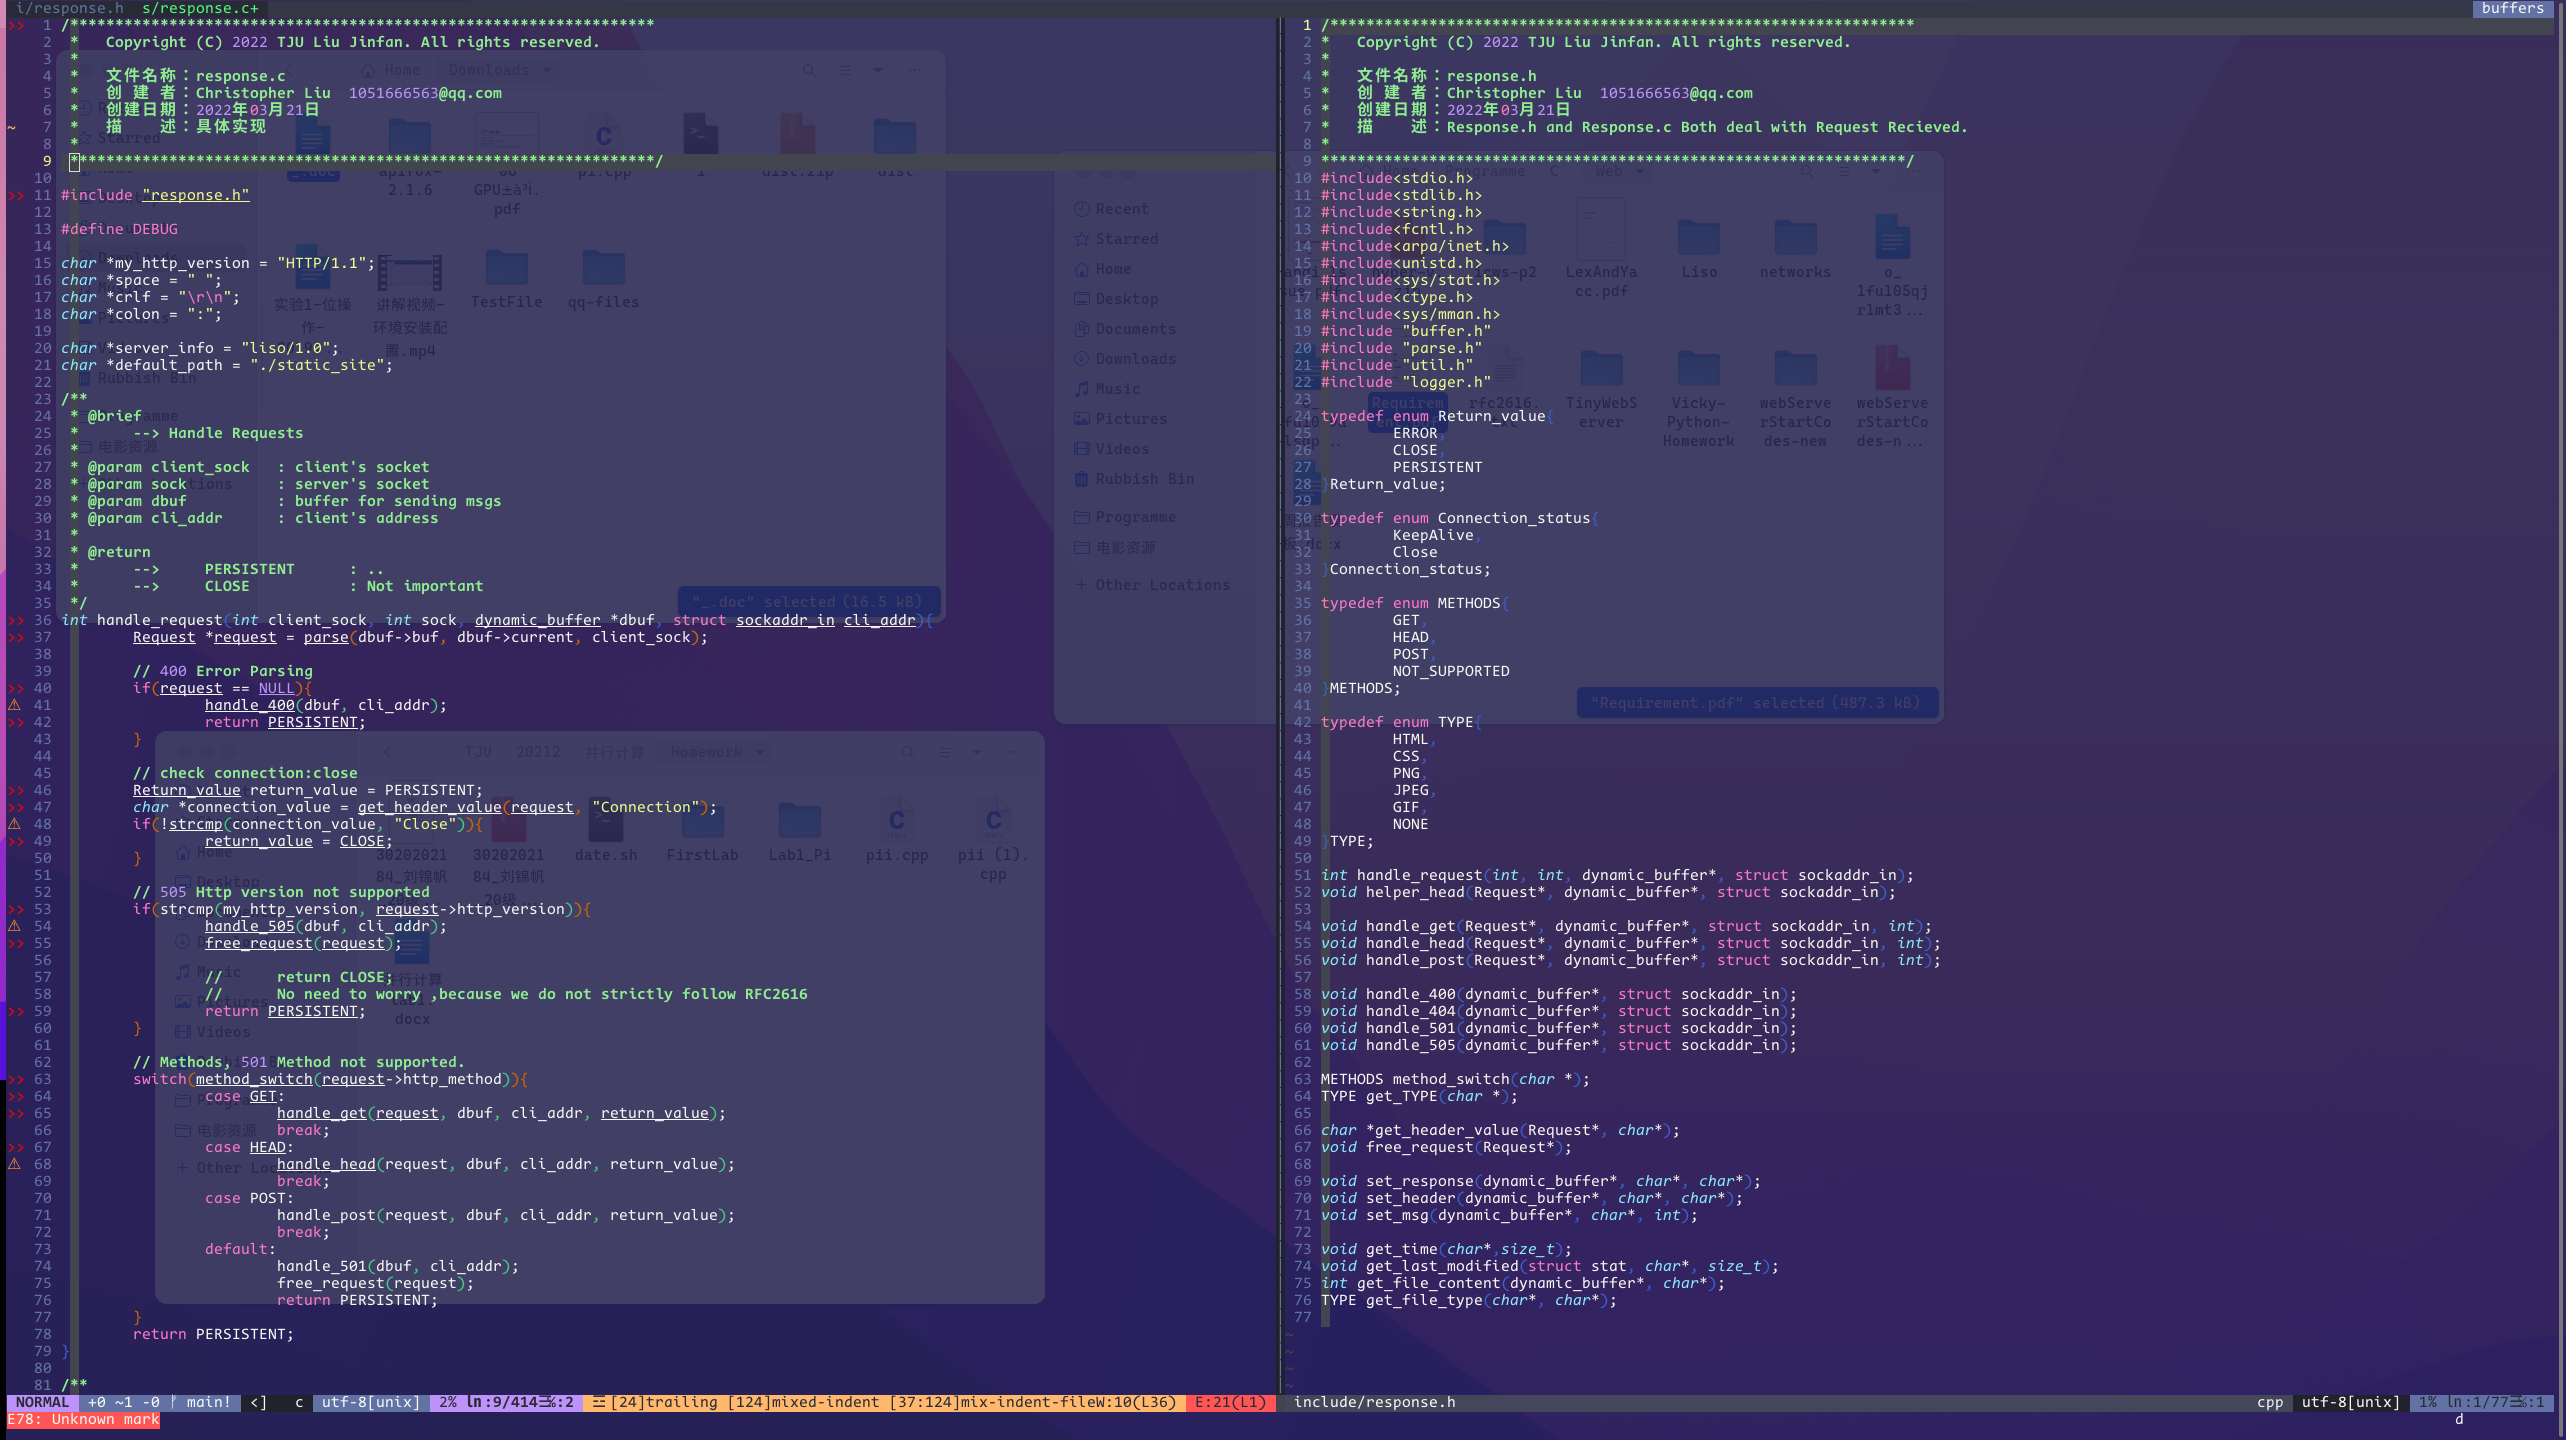
\includegraphics[width=5in]{responsech.png}}
    \subfigure[liso\_server.c 和 liso\_client.c]{\label{fig:liso}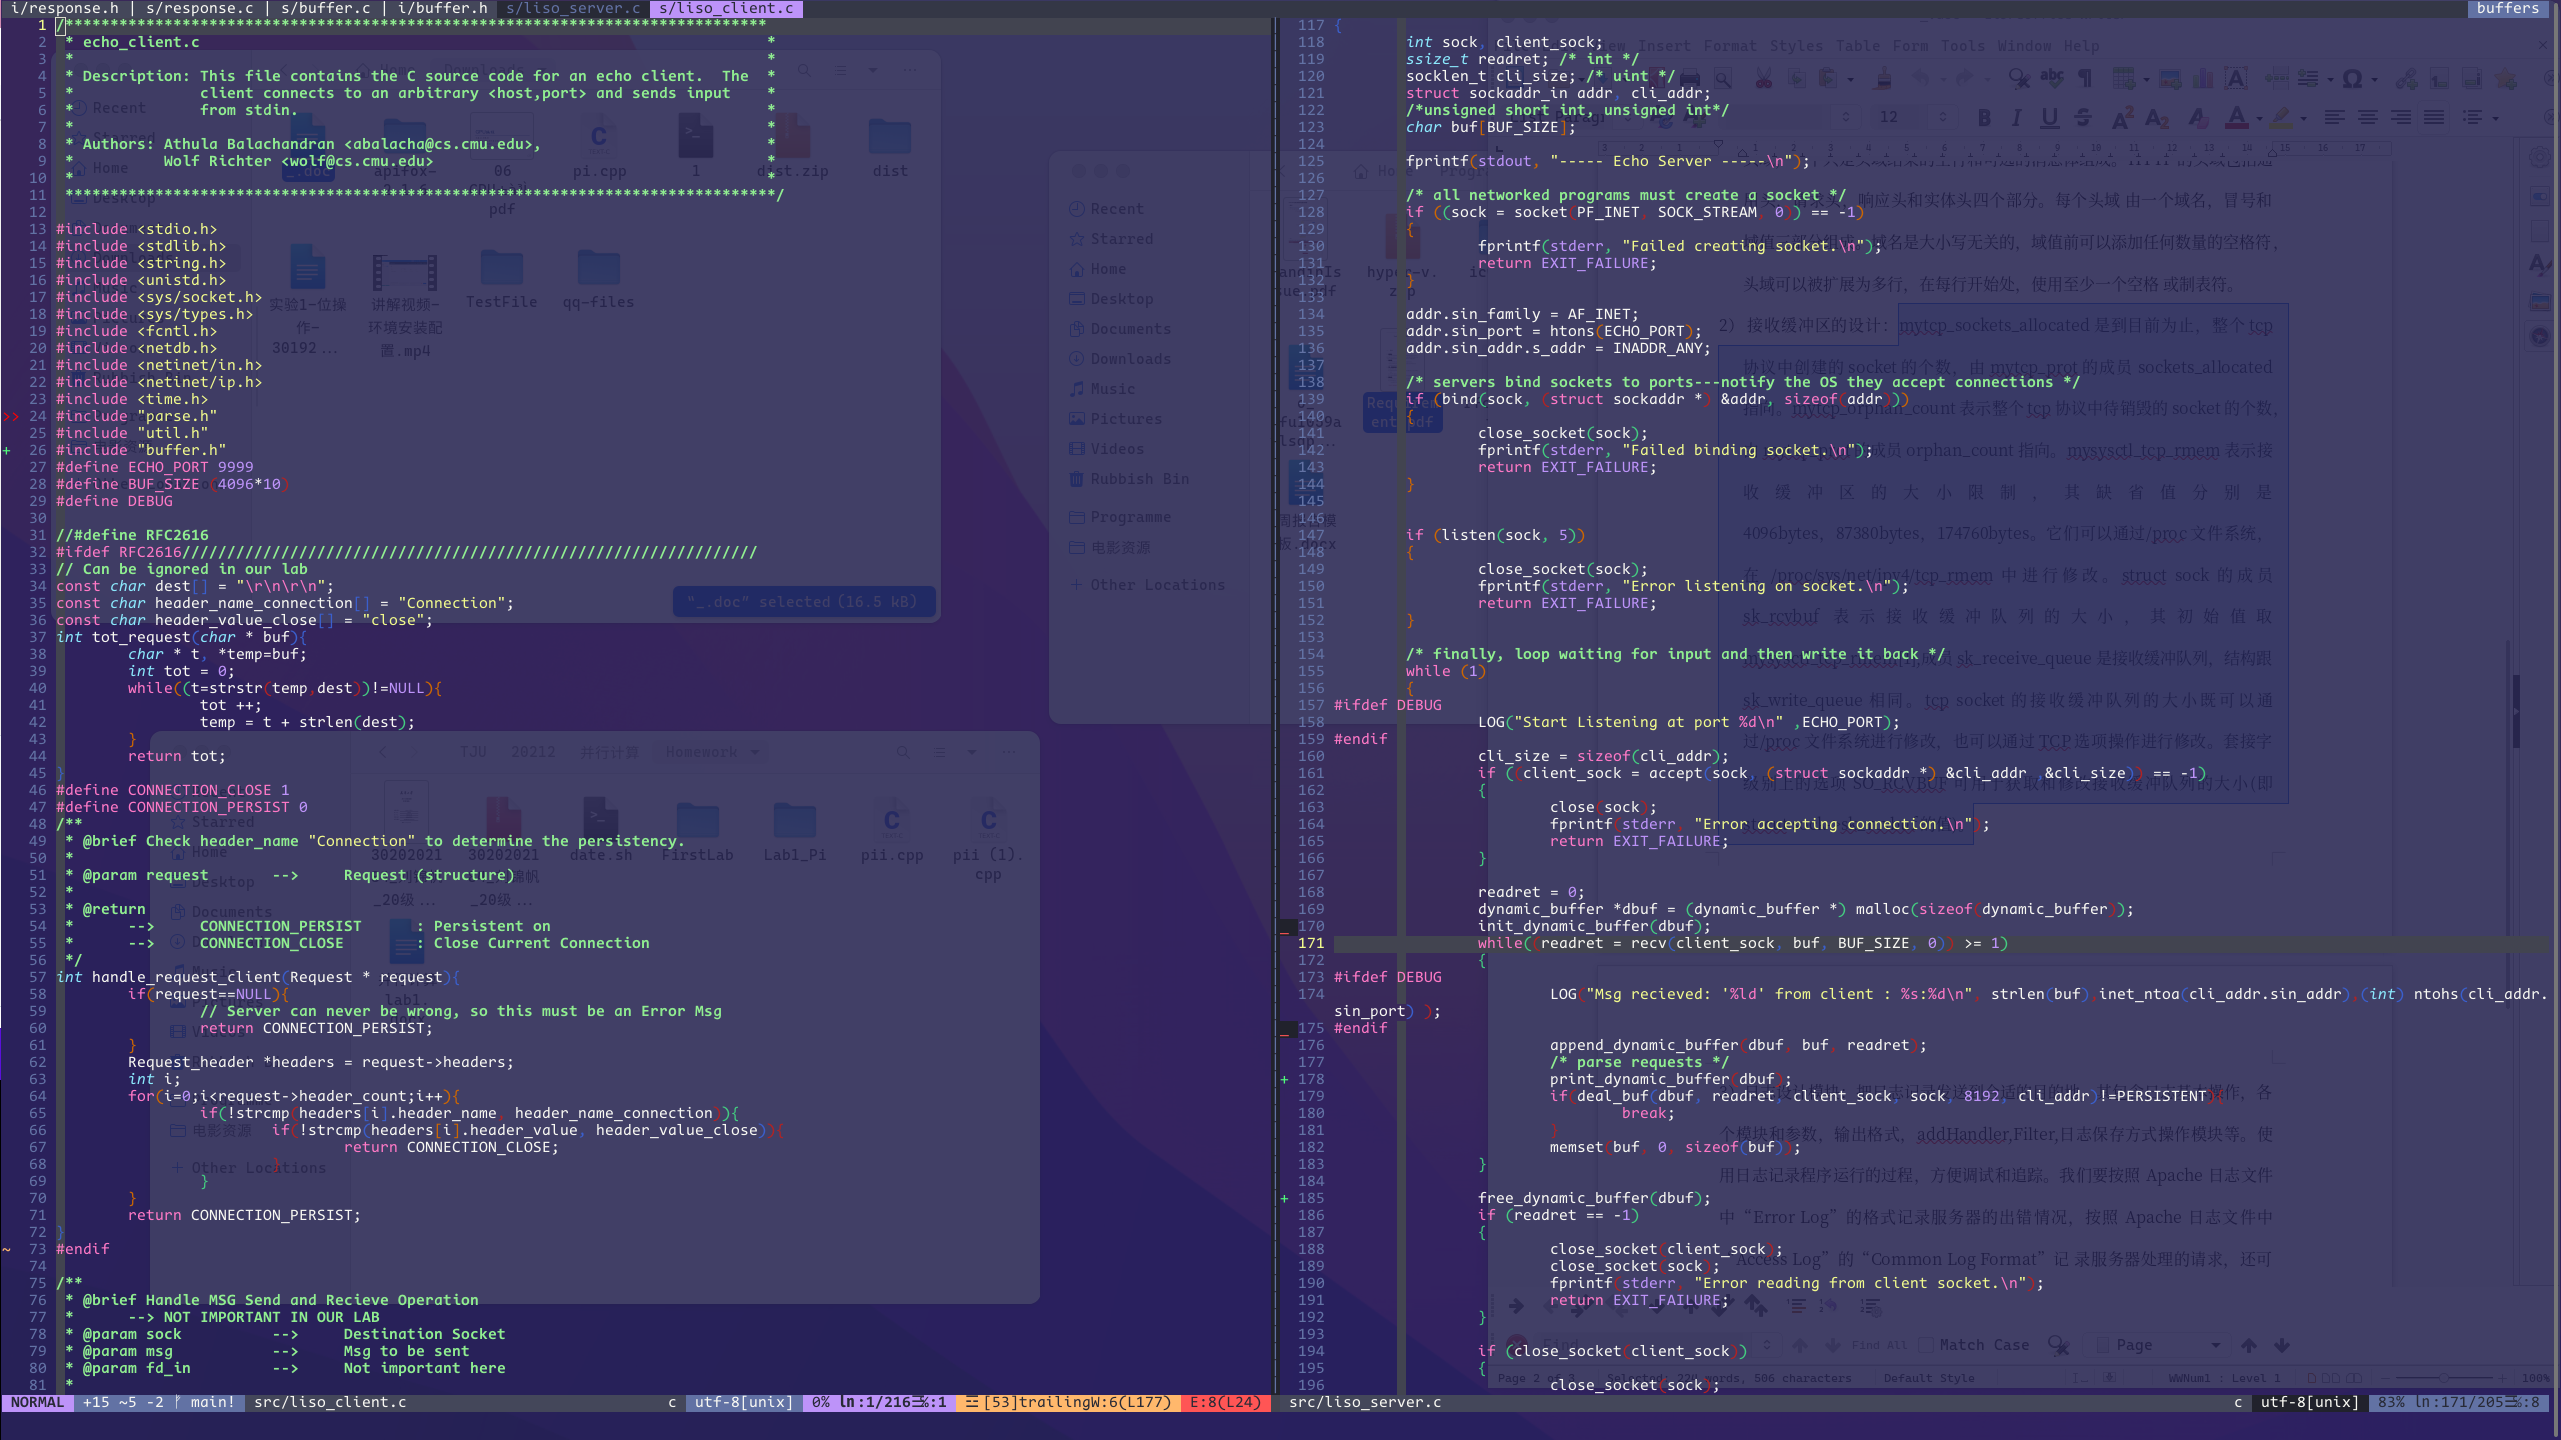
\includegraphics[width=5in]{liso.png}}
    \caption{核心代码}\label{fig:Main}
\end{figure}

\paragraph*{GET} GET 方法在 HEAD 方法的基础之上,添加了读取文件的操作,根据模块化变成的思想,我们将其封装到函数 get\_file\_content() 之中。为了实现对缓冲区的管理、避免 Segment Fault,我们仍先通过 stat 函数对文件情况做初步确定,并先对动态数组进行扩容,再读入文件。文件读入部分将在后续小节进行介绍。

\paragraph*{POST} POST 方法的实现,根据实验要求,直接返回接收到的报文,于是在判断没有 400,505,以及 501 错误之后,我们即可将携带请求信息的动态数组 dbuf 原路返回。

\section{妥善管理缓冲区}

由于 socket 编程本身的性质,在 send 函数中会主动的将信息拆分成合适大小再分别发送。所以我们只需要针对 \textbf{1.} 发送前,用户的缓冲区; \textbf{2.} 接收后集中存放的用户缓冲区; 两个缓冲区进行管理。

\subsection{动态数组定义与实现}
我们的策略,是通过自定义的动态数组实现对一个动态长度的缓冲区的支持。具体定义及部分实现如图\ref{fig:dynamicBuffer}所示。


部分结构体、函数介绍如下:

\paragraph*{struct dynamic\_buffer} 该结构体定义了一个基地址 *buf, 以及它的总大小 capacity 和当前大小 current。

\paragraph*{init\_dynamic\_buffer()} 该函数使用系统调用 malloc 将为一个新定义的动态数组分配由宏 "DEFAULT\_CAPACITY" 定义的空间。即对动态数组进行初始化。

\paragraph*{append\_dynamic\_buffer()} 该函数将一个字符串拼接到动态数组后面。首先判断当前空间是否够用,如果不够,则调用函数 realloc 为其增添空间,然后通过 memcpy() 函数,将新添加的字符串拼接到动态数组后面。


\subsection{动态数组使用}

动态数组的作用是解决缓冲区溢出问题,前文提到的两个可能出现溢出的地点,分别是读入文件时由于文件过大(或将其加入返回信息时)而溢出,另一个是在接收端虽然一次性接收的最大值由 BUF\_SIZE 控制,但是用户发送的请求大小不可定(例如 Lab3 中的 pipeline),导致缓冲区溢出。最终为了整体的和谐性,我们在大多数使用字符串数组的地方,都改用我们的动态数组。例如:

\paragraph*{读入文件时} 首先使用 stat() 获取文件大小,然后调用函数 add\_dynamic\_buffer() 函数对我们的动态数组进行可用空间的检验。最后再通过 read() 或者 mmap() 将文件写入动态数组。

\paragraph*{Server 端} 在 server 端,我们使用动态数组,存储即将返回给 client 的信息。由于 GET 可能会请求大小超标的文件,于是我们通过有保护机制的动态数组,安全地对它进行读取与返回。

\paragraph*{接收 socket 信息时} 由前文提到地 recv() 函数的性质,我们知道应该通过 while 来不断读取管道里的信息,如图\ref{fig:liso} 右侧第 171 行。通过 append\_dynamic\_buffer() 函数,将读取的信息添加到当前动态数组 dbuf 中。每次处理缓冲区,即是对 dbuf 中的数据进行拆分(确定一份请求报文)、解析与返回,最后调用 update\_dynamic\_buffer() 函数,将该报文从动态数组中丢弃。最大限度地节约空间,并解决缓冲区溢出问题。
\begin{figure}[htbp!]
    \centering
    \subfigure[dynamic\_buffer.c 和 dynamic\_buffer.h]{\label{fig:dynamicBuffer}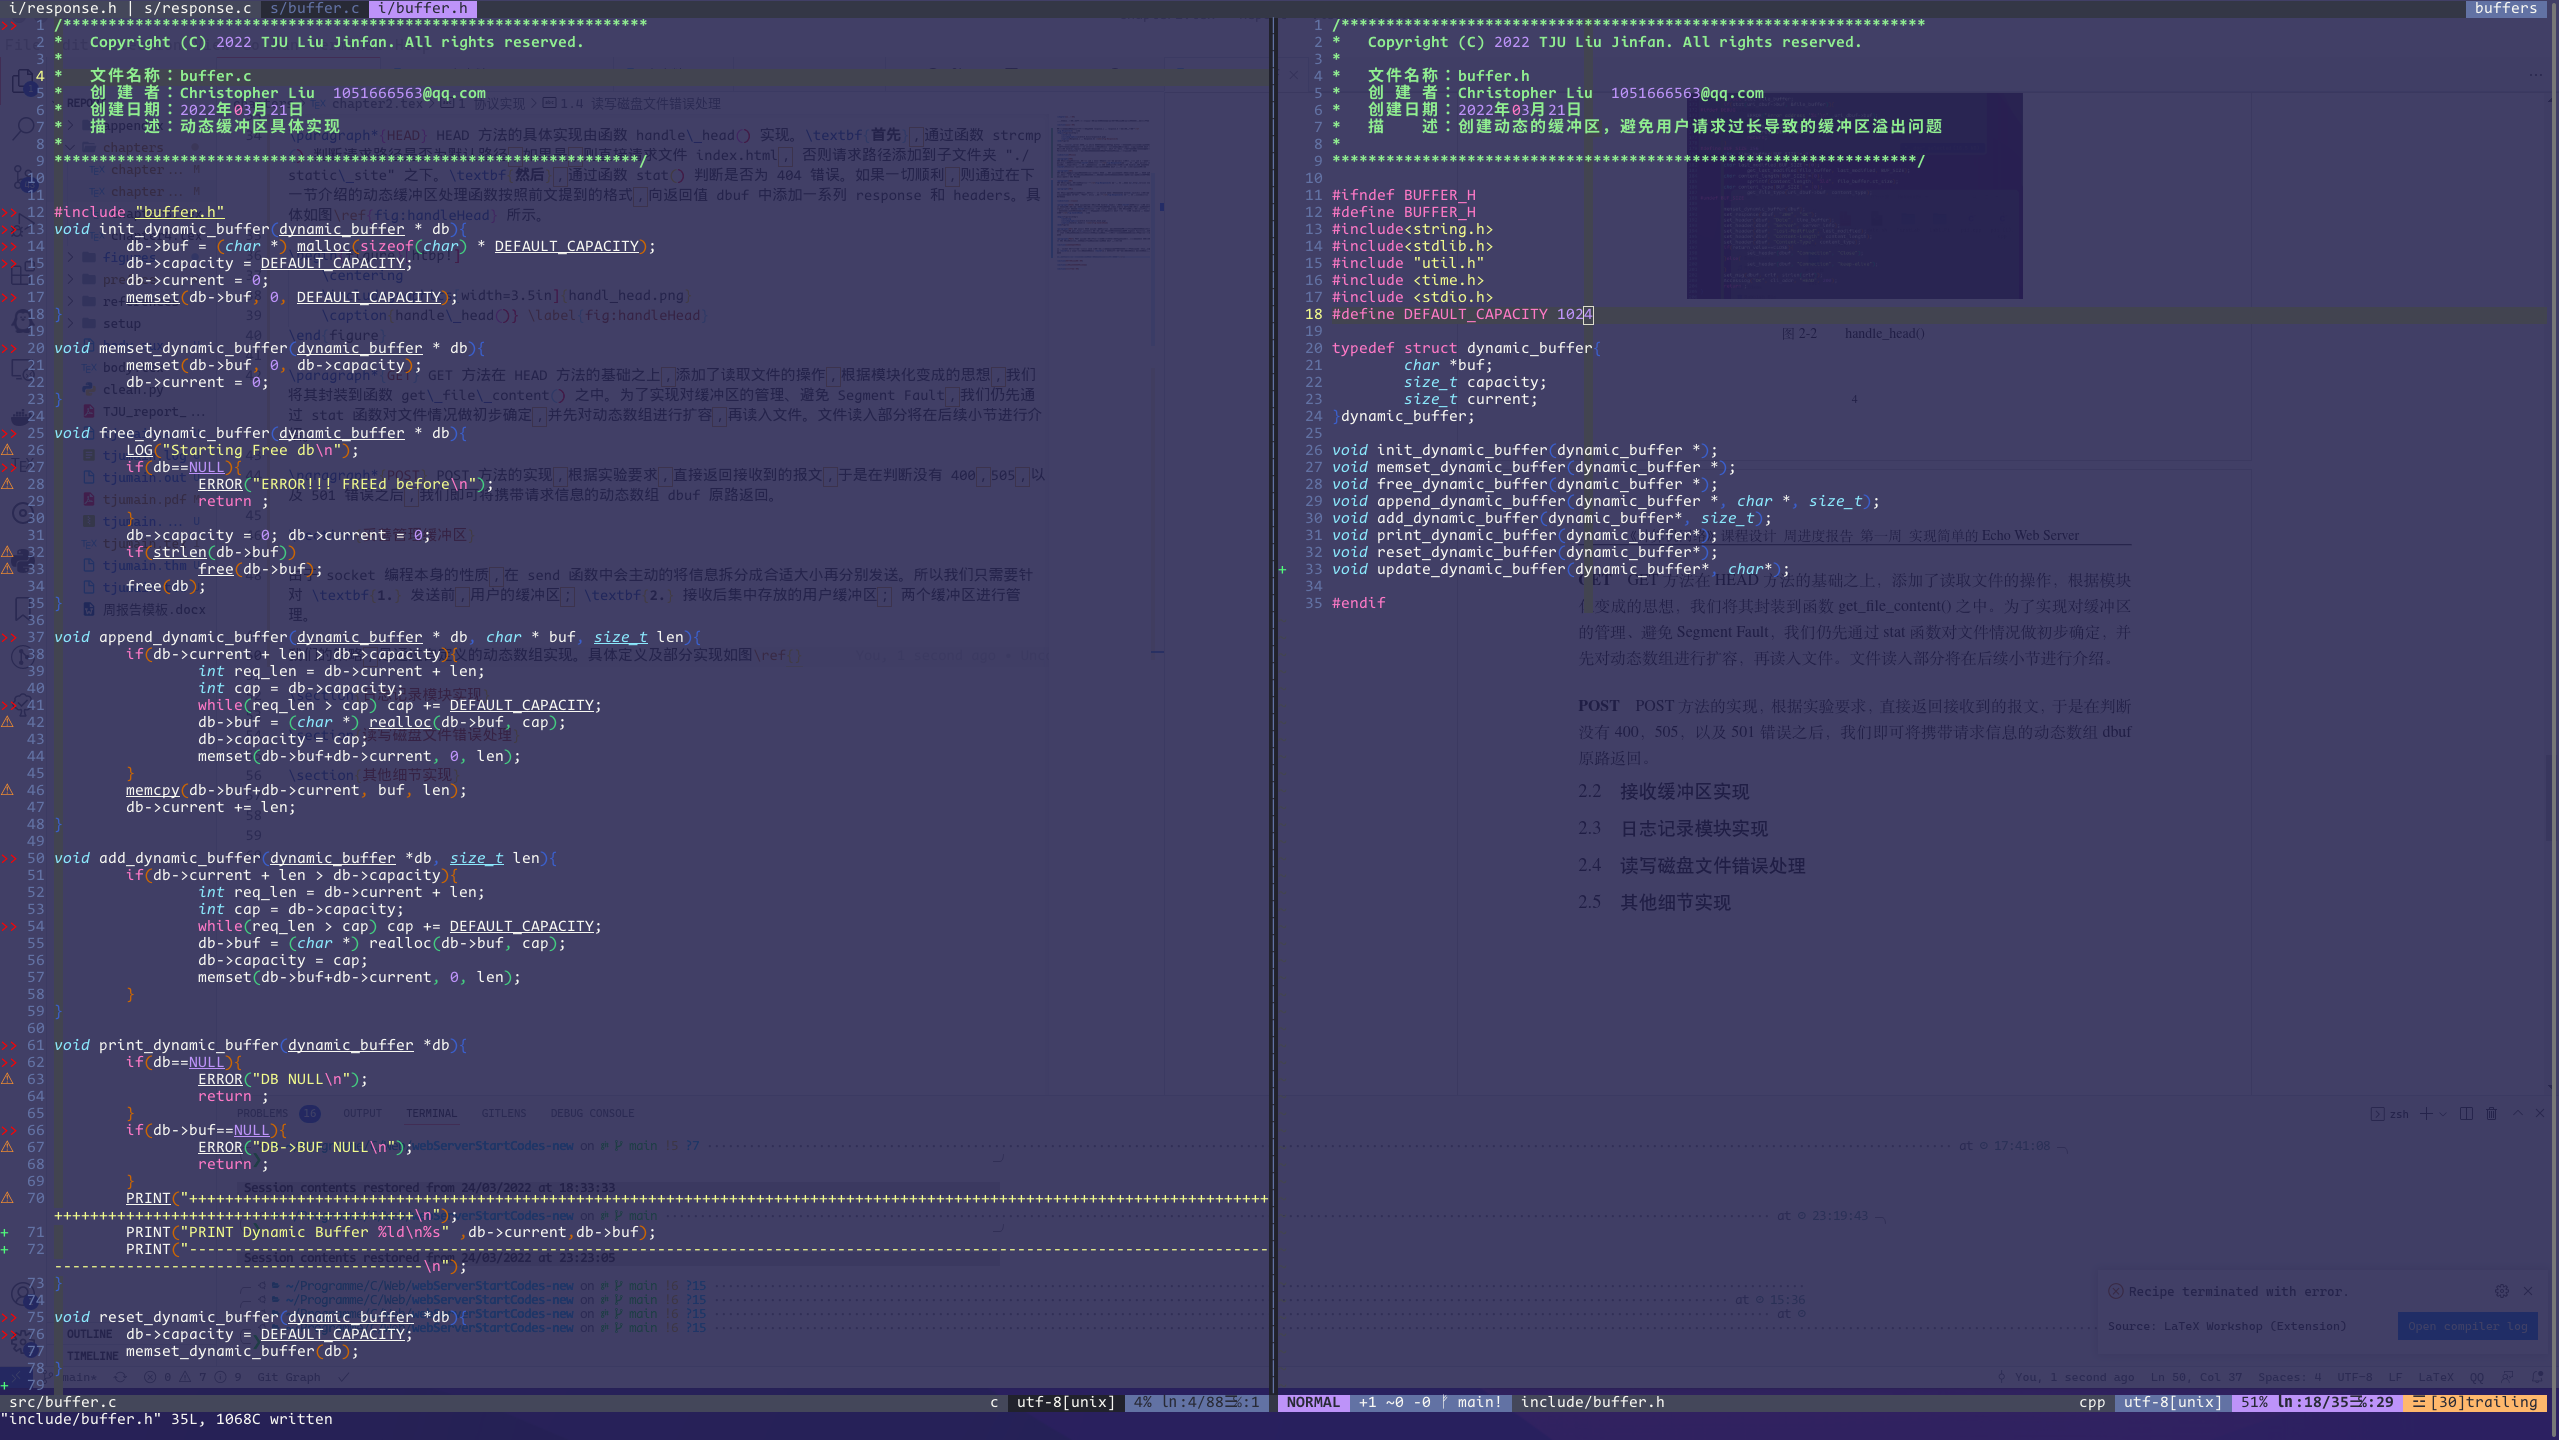
\includegraphics[width=5.5in]{dynamic_buffer.png}}
    \subfigure[handle\_head 函数]{\label{fig:handleHead}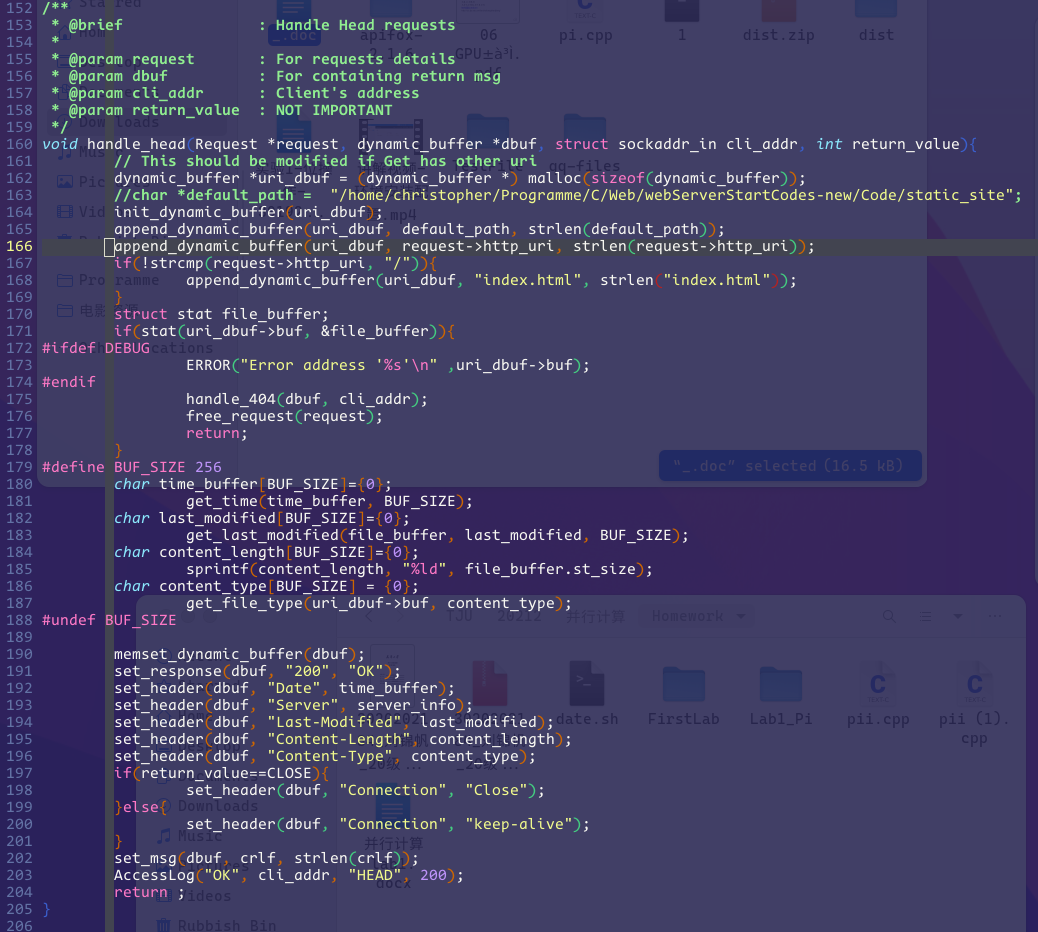
\includegraphics[width=2.1in]{handl_head.png}}
    \subfigure[日志文件]{\label{fig:log}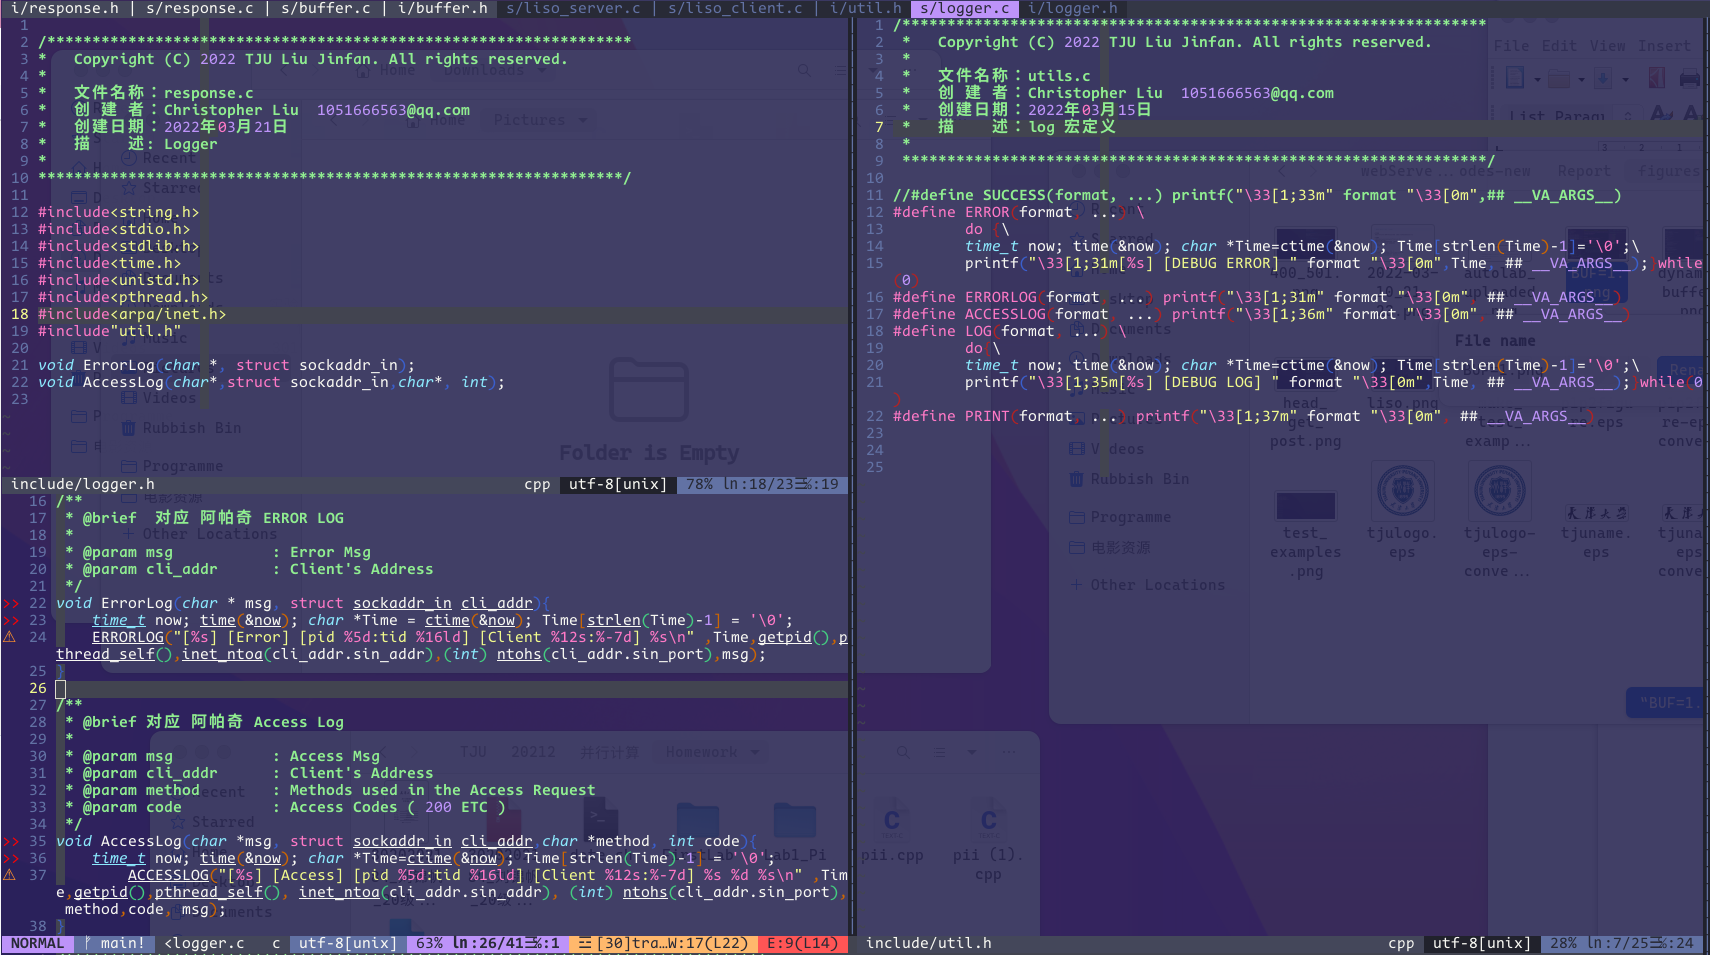
\includegraphics[width=3.3in]{log.png}}
    \caption{动态数组、日志文件以及 Handle Head 函数}\label{fig:Chapter2}
\end{figure}


\subsection*{验证}
如图\ref{fig:buffer},即使将缓冲区大小设置为 1,我们的 server 依旧正常处理并返回信息(测试样例为 pipeline,由于和 Persistent Connection 相关联,故一起实现了)。

% \begin{figure}[htbp!]
%     \centering
%     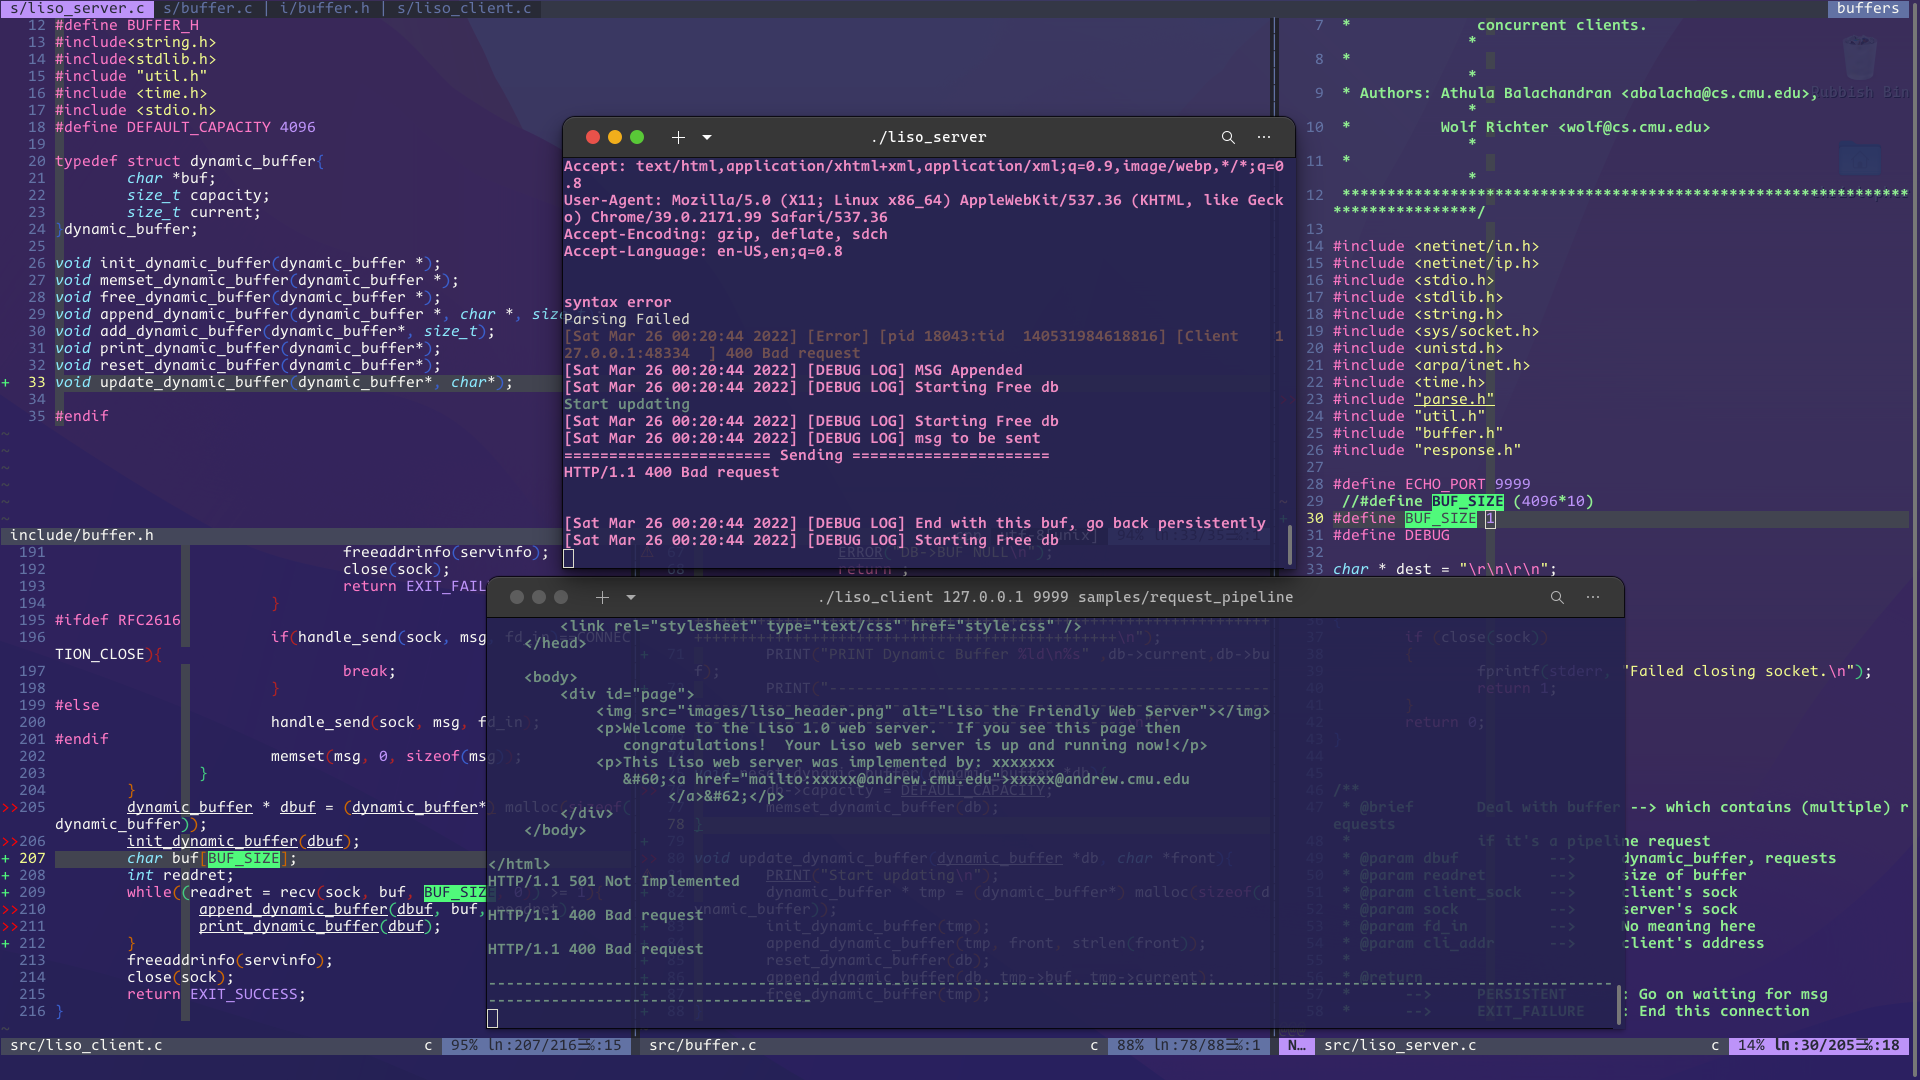
\includegraphics[width=4.4.5in]{BUF=1.png}
%     \caption{buffer test, BUF\_SIZE = 1}\label{fig:buffer}
% \end{figure}

\begin{figure}[htbp!]
    \centering
    \subfigure[buffer\_test,BUF\_SIZE=1]{\label{fig:buffer}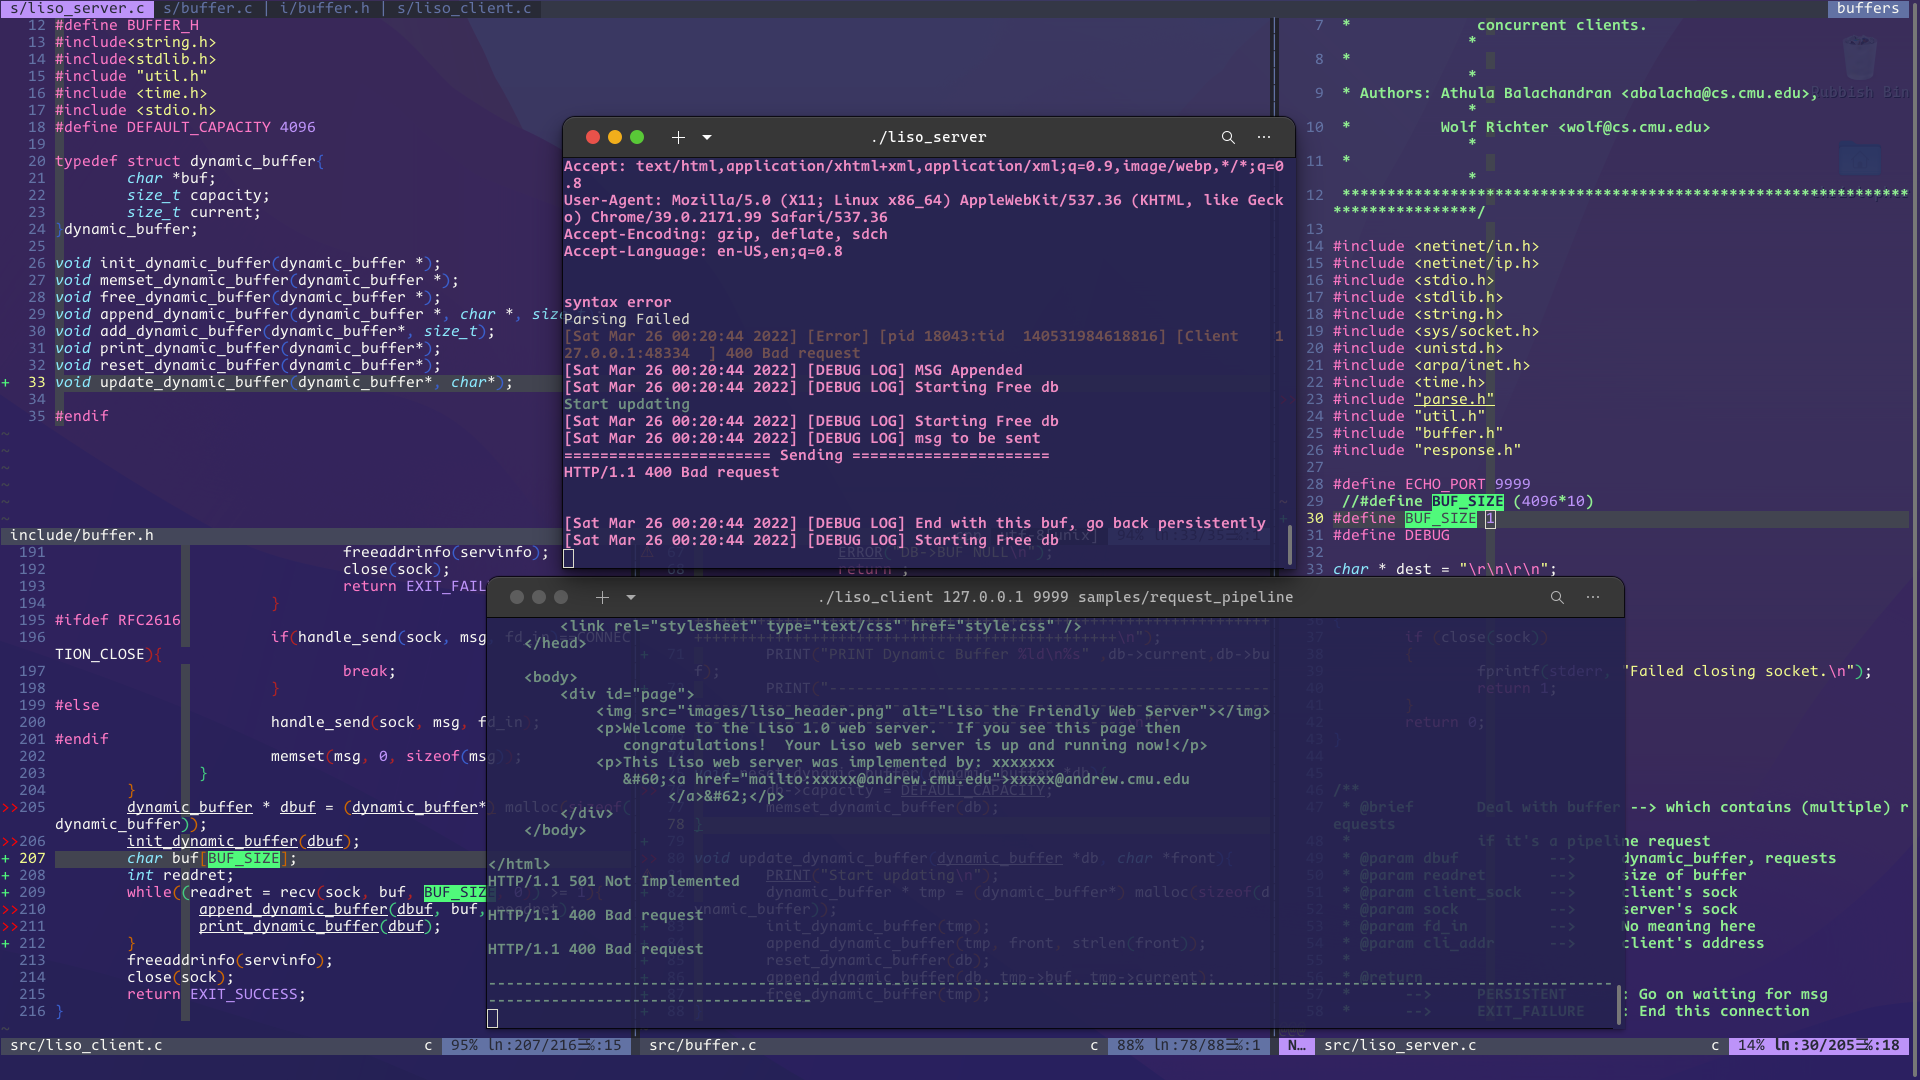
\includegraphics[width=3.5in]{BUF=1.png}}
    \subfigure[get\_file\_content函数]{\label{fig:openfile}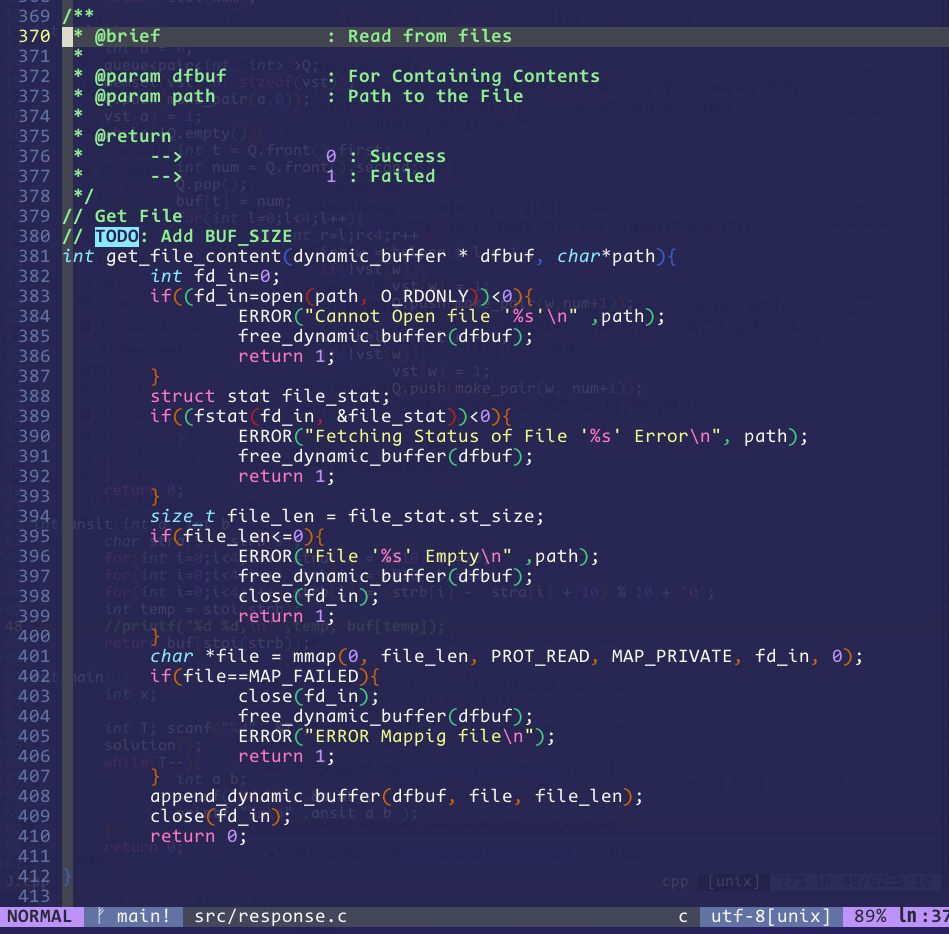
\includegraphics[width=2in]{getFileContent.png}}
    \caption{测试 buffer 以及 get\_file\_content 函数}\label{fig:Chapter2.2}
\end{figure}

\section{日志记录模块实现}
日志记录模块借用了 Apache 标准,使用 C 宏定义完成第一层封装,采用 logger.c 与 logger.h 配合,进行向特定文件的输入,实现了 log 的可跟踪性。具体宏定义如图\ref{fig:log} 所示。

\section{读写磁盘文件错误处理}
只有 GET 和 HEAD 请求涉及对文件的处理。根据之前的描述,我们首先使用 stat() 函数对磁盘文件进行试探性的访问。如果在此时出错,可能有 1. 路径不存在; 2. 没有查看权限。在服务器看来,我们只需返回 404 错误即可。

在 GET 的处理中,我们还需对文件进行读取,此时可能又会产生 3. 无法打开的错误; 4. 文件为空;以及 5. 无法正确映射到内存;等问题(由于我们使用了上一节提到的动态数组,不会存在溢出问题)。

考虑完上述问题,我们实现了如图\ref{fig:openfile} 的代码。

% \begin{figure}[htbp!]
%     \centering
%     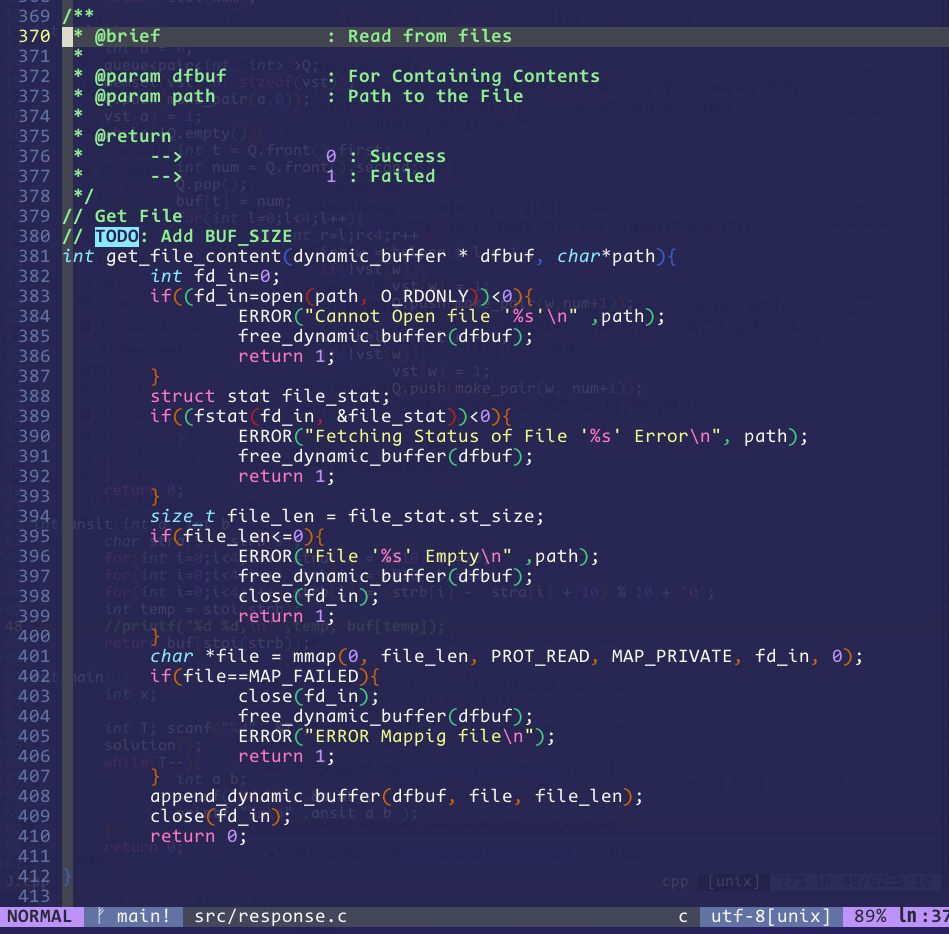
\includegraphics[width=2.5in]{getFileContent.png}
%     \caption{get\_file\_content 函数}\label{fig:openfile}
% \end{figure}